\documentclass{segabs}
\usepackage{xspace,color,amsmath}
\usepackage{amssymb}
\usepackage{hyperref}
\begin{document}
\title{A 3D finite volume approach for time-domain electromagnetic simulations with thin, highly conductive structures}
\author{
Devin C. Cowan$^1$, Lindsey J. Heagy$^1$, Douglas W. Oldenburg$^1$ \\
$^1$Geophysical Inversion Facility, University of British Columbia \\
}
\email{devin.cowan@ubc.ca}
% \footer{Example}
%\lefthead{Cowan, Heagy \& Oldenburg}
%\righthead{Influence of transfer functions on airborne magnetotelluric inversion}
\maketitle

\begin{abstract}

\vspace{-15pt}
Inductive source time-domain electromagnetic (TDEM) methods are frequently used to image ore-bearing mineralization that can present as thin and highly conductive. The need to properly characterize inductive responses from thin, highly conductive targets in geologically complex settings has promoted significant interest in developing improved numerical algorithms. Here, we present a 3D hierarchical finite volume (FV) formulation that accurately simulates the physics of thin conductors without undo computational cost. The formulation parameterizes the electrical properties of plate-like structures as conductances that live on mesh faces. We build the formulation using the SimPEG framework. We show the hierarchical FV approach better preserves the physics of the forward simulation compared to plate-modeling software while using a fraction of the computational resources required for standard 3D voxel approaches. We demonstrate the hierarchical FV approach to be numerically stable for plate conductances exceeding 1e4 S. We then demonstrate the simulation of borehole TDEM data where the geometry of the host and a conductive target are non-trivial, and the electrical properties of the target are inhomogeneous. The impact of the hierarchical FV formulation is the ability to perform hypothesis testing for geologically realistic hypotheses when thin conductive targets are present.
\end{abstract}

\vspace{-15pt}
\section{Introduction}

Inductive source time-domain electromagnetic (TDEM) methods are frequently used to image ore-bearing mineralizations that can present as thin and highly conductive. TDEM responses from these targets have historically been characterized with plate-modeling approaches \citep{HannesonWest1984,WalkerLamontagne2006}. However, plate modeling codes are limited in their ability to model 3D heterogeneous geology. 3D voxel-based approaches are not limited by geological complexity. However, the computational cost of 3D voxel-based algorithms becomes prohibitive when targets are sufficiently thin and/or conductive. The need to properly characterize inductive TDEM responses from thin, highly conductive targets ($>$1e4 S/m) within geologically complex settings has promoted significant interest in developing improved numerical algorithms.

Progress has been made in the development of 3D voxel-based algorithms for imaging thin and highly conductive structures. \citeyear{Weiss2017} developed a finite element approach to solve the DC resistivity problem, wherein model parameters defining plate-like structures are parameterized to mesh faces and model parameters defining wire-like structures are parameterized to mesh edges. \citeyear{Hu2022} adapted the original concept to develop a finite volume (FV) approach for well-casing applications in the frequency-domain. However, previous studies do not include TDEM problems and consider only galvanic sources.

In this abstract, we augment the FV approach described in \citep{Haber2014} to simulate inductive source TDEM data in the presence of thin, highly conductive structures. We do this by augmenting the inner-product matrix obtained from Ohm's law to include contributions from volumetric currents that live within cells, surface currents that live on cell faces and line currents that live on cell edges. This hierarchical FV formulation is implemented using the SimPEG \citep{Cockett2015} framework. In this abstract, our study is limited to problem geometries that include volumetric and surface currents. For a coincident loop airborne survey configuration, we simulate TDEM data over a thin, dipping conductor within a resistive halfspace.  Simulation results using hierarchical FV are compared against a highly discretized standard FV approach and the P223 suite LEROI plate-modeling code \citep{Raiche2007}. We demonstrate the stability of the hierarchical FV approach as the conductance of the target exceeds 1e4 S. We then demonstrate the simulation of borehole TDEM data where the geometry of the host and thin conductor are non-trivial, and the electrical properties of thin conductor are inhomogeneous.


%========================================================
\section{Hierarchical Finite Volume Method}
%========================================================

The FV method solves Maxwell’s equations approximately on a numerical grid (mesh) while preserving mimetic properties of the governing partial differential equations. Applying the standard FV approach and using natural boundary conditions, the time-dependent weak form solution for the electric fields $\mathbf{e}$ discretized to mesh edges is given by \citep{Haber2014}:
\begin{equation}
\mathbf{C^T M_{f\mu} C e} + \mathbf{M_{e\sigma}} \frac{\partial \mathbf{e}}{\partial t} = - \frac{\partial \mathbf{s_e}}{\partial t}
\label{eq:e_formulation}
\end{equation}
where electric displacement is ignored. For magnetic flux densities $\mathbf{b}$ discretized to mesh faces, the solution is given by:
\begin{equation}
\mathbf{C^T M_{e\sigma}^{-1} C M_{f\mu} b} + \frac{\partial \mathbf{b}}{\partial t} = - \mathbf{C^T M_{e\sigma}^{-1} s_e}
\label{eq:b_formulation}
\end{equation}
$\mathbf{C}$ is the discrete curl operator from edges to faces, $\mathbf{M_{e}}$ is the inner-product matrix for vectors discretized to edges, $\mathbf{M_{e\sigma}}$ is the inner-product matrix for electrical conductivities $\sigma$ projected to edges, $\mathbf{M_{f\mu}}$ is the inner-product matrix for inverse magnetic permeabilities $\mu$ projected to faces, and $\mathbf{s_e}$ is an integrated electrical source term. In SimPEG, Eqs. \ref{eq:e_formulation} and \ref{eq:b_formulation} are solved using backward Euler at a discrete set of time-steps.

\begin{figure}
\centering
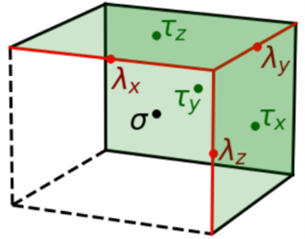
\includegraphics[width=0.4\columnwidth]{images/hierarchical_properties.png}
\caption{Discretization of volume conductivities ($\sigma$), face conductances ($\tau_x , \tau_y , \tau_z$) and integrated conductivities on edges ($\lambda_x , \lambda_y , \lambda_z$).}
\label{fig:hierarchical_properties}
\end{figure}

For the hierarchical FV approach, we define a new parameterization for the Earth's electrical properties by decomposing the current density into volumetric currents that live within cells, surface currents that live on cell faces and line currents that live on cell edges. When taking the inner-product between a test function $\vec{u}$ and Ohm's law, we obtain:
\begin{equation}
\begin{split}
\label{eq:sum}
\int_\Omega \, \vec{u} \cdot \vec{j} \,  dv = & \sum_k^{nC} \, \int_{V_k} \, \vec{u} \cdot \sigma_k \vec{e} \, dv \\
&+ \sum_k^{nF} \, \int_{A_k} \, \vec{u} \cdot \tau_k \vec{e} \, da \\
&+ \sum_k^{nE} \, \int_{L_k} \, \vec{u} \cdot \lambda_k \vec{e} \, d\ell
\end{split}
\end{equation}
where $\sigma_k$ defines the conductivity within cell k, $\tau_k$ defines the conductance for face k, and $\lambda_k$ defines the conductivity integrated over the cross-sectional area of a wire element that lives on edge k. Figure \ref{fig:hierarchical_properties} illustrates where volume, face and edge properties live. Assuming cell faces and edges are infinitesimally thin, surface currents normal to surfaces and edge currents normal to edges are negligible. The discrete relationship between the current density and the electric field can be defined as:
\begin{equation}
\label{eq:hierarchical}
\int_\Omega \, \vec{u} \cdot \vec{j} \,  dv \approx \big [ \mathbf{M_{e\sigma} + M_{e\tau} + M_{e\lambda}} \big ] \, \mathbf{e}
\end{equation}
where $\mathbf{M_{e\tau}}$ is the inner-product matrix for face conductivities projected to edges and $\mathbf{M_{e\lambda}}$ is the inner-product matrix for the electrical properties of the wire elements projected to edges. To account for the face and edge currents, the hierarchical formulation replaces $\mathbf{M_{e\sigma}}$ with $\mathbf{M_{e\sigma}+M_{e\tau}+M_{e\lambda}}$ in Eqs. \ref{eq:e_formulation} and \ref{eq:b_formulation}.



%========================================================
\section{Airborne TDEM for a thin dipping conductor}
%========================================================

Here, we simulate coincident loop airborne TDEM data over a thin dipping conductor within a resistive halfspace (Figure \ref{fig:airborne_geometry}). We simulate and compare both vertical b-field and db/dt data using: 1) a highly discretized standard FV approach, 2) a more coarsely discretized hierarchical FV approach, and 3) plate-modeling with LEROI. The transmitter waveform is a square pulse with a 0.01 s on-time. The host is given a conductivity of 1e-4 S/m. The dipping conductor is rectangular with a side length of 80 m, a thickness of 6 m, and dips 45 degrees to the East. The plate has an electrical conductivity of 16.6 S/m so that it has a conductance of 100 S.


\begin{figure}
\centering
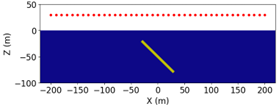
\includegraphics[width=0.6\columnwidth]{images/airborne_geometry.png}
\caption{Coincident loop airborne survey geometry.}
\label{fig:airborne_geometry}
\end{figure}

\begin{figure}
\centering
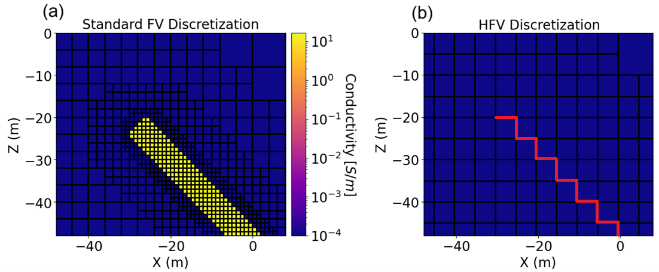
\includegraphics[width=\columnwidth]{images/airborne_discretization.png}
\caption{(a) Discretization and conductivity model used for the standard FV simulation. (b) Discretization and step-projection of 100 S conductance plate to faces for the hierarchical FV simulation.}
\label{fig:airborne_discretization}
\end{figure}

For the highly discretized standard FV approach, a minimum cell size of 1 m was required near the target to accurately simulate the physics (Figure \ref{fig:airborne_discretization}a). This resulted in an OcTree mesh with 153,899 total cells. While this approach is expected to be the most accurate, the required memory exceeded 16 GB. For the LEROI simulation, the target is parameterized as a 100 S plate conductor within a 1e-4 S/m halfspace. Using 5 m wide square tiles to discretize the plate, the memory requirements for the simulation were negligible, and the run time was several minutes. For the hierarchical FV approach, a minimum cell size of 10 m is used to generate the OcTree mesh, resulting in 58,612 total mesh cells. The electrical properties of the host are defined as 1e-4 S/m conductivities at cell centers. The target is defined as a 100 S plate conductor. A step projection is used to map the 100 S conductance plate to the appropriate mesh faces (Figure \ref{fig:airborne_discretization}b). The hierarchical FV simulation required $<$4 GB of memory and was run in ~5 min on a laptop.

Figure \ref{fig:airborne_comparison} shows the comparison between the three simulations. While LEROI boasts the shortest run-time, it does not account for EM interactions between the target and the air-Earth interface. Consequently, the target response does not match the highly discretized FV simulation. The hierarchical FV approach is generally able to reproduce the expected b-field and db/dt data while requiring only moderate computational resources.


\begin{figure}
\centering
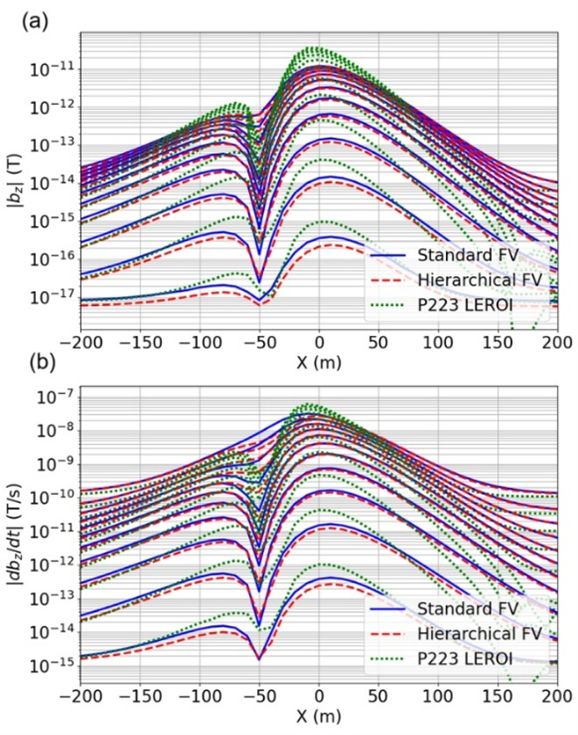
\includegraphics[width=0.65\columnwidth]{images/airborne_comparison.png}
\caption{Comparison between standard FV, hierarchical FV and P223 LEROI for a coincident loop airborne TDEM line (a) b-field data. (b) db/dt data.}
\label{fig:airborne_comparison}
\end{figure}

%========================================================
\section{Simulation for high conductors}
%========================================================

Here, we demonstrate the stability of the hierarchical FV approach for high conductors. We reuse the problem geometry and 58,612 cell OcTree mesh from the previous section. For plate conductances of 1e2 S, 1e5 S and 1e8 S, we use the hierarchical FV approach to simulate the data.

Simulation results are shown in Figure \ref{fig:airborne_high_conductor}. While the b-field and db/dt data for the 1e2 S target decays over the simulated range of time channels, the 1e5 S target shows a static signature in the b-field data and does not present until later times in the db/dt data. Since the decay constant for the 1e8 S target is so large, the b-field response does not appear until later times and the db/dt data are insensitive to the target, as expected.

\begin{figure}
\centering
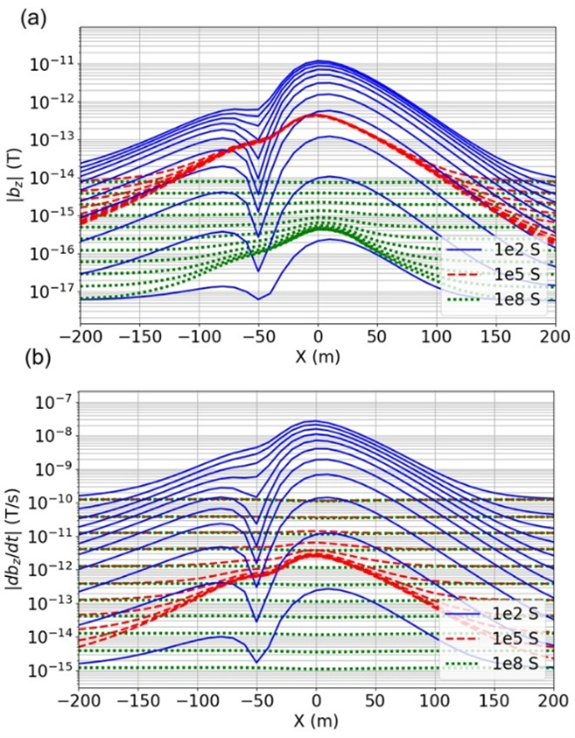
\includegraphics[width=0.65\columnwidth]{images/airborne_high_conductor.png}
\vspace{-10pt}
\caption{Hierarchical FV simulation for high conductances. (a) b-field data. (b) db/dt data.}
\label{fig:airborne_high_conductor}
\vspace{-5pt}
\end{figure}

%========================================================
\section{TDEM simulation for a complex setting}
%========================================================

Here, we simulate borehole University of Toronto EM (UTEM) data where the geometry of the host and a thin conductive target are non-trivial, and the electrical properties of the target are inhomogeneous. Our simulation example is inspired by the Voisey’s Bay Eastern deeps magmatic Ni-Cu-Co deposit.

We consider the synthetic problem geometry illustrated in Figure \ref{fig:utem_geometry}, wherein the Earth is excited with a 1,200 m wide square transmitter loop with a 1 Hz operating frequency. We simulate channel reduced data for channels 1 (0.25 s) through 8 (0.001953 s) for three boreholes. For the background conductivity model, we define the electrical properties of a highly resistive basement (2.5e-5 S/m), a troctolite chamber (2.5e-4 S/m), and a portion of the troctolite chamber that hosts weaker mineralization (1e-2 S/m). We use the triangles of a 3D Delaunay surface to define variable conductance along a sheet-like target characterizing massive sulphide mineralization. A step projection is used to map the conductances to the faces of an OcTree mesh for the simulation. Figure \ref{fig:utem_discretization} shows the non-zero conductances defined on mesh faces.

\begin{figure}
\centering
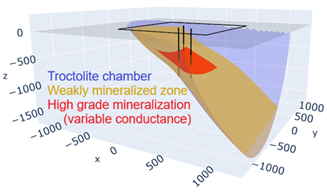
\includegraphics[width=0.65\columnwidth]{images/utem_geometry.png}
\caption{Borehole UTEM simulation geometry.}
\label{fig:utem_geometry}
\end{figure}

\begin{figure}
\centering
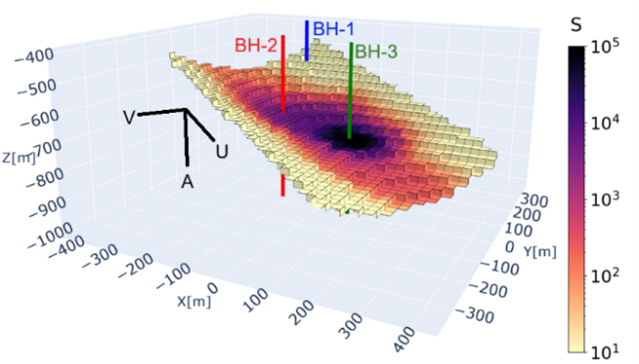
\includegraphics[width=0.65\columnwidth]{images/utem_discretization.png}
\caption{Conductances projected to mesh faces and borehole-centric coordinate directions U, V and A.}
\label{fig:utem_discretization}
\end{figure}

Channels 1 through 8 of the simulated channel reduced data for BH-1 are plotted in Figure \ref{fig:utem_bh1}. The sign of the A-component signature indicates the borehole lies outside a dominant conductor. U and V-component signatures indicate the dominant conductor is offset in both the down-dip and cross-line directions. The simulated channel reduced data for BH-2 are plotted in Figure \ref{fig:utem_bh2}. The signatures indicate the borehole intersects a significant conductor at a depth of ~650 m. The simulated channels reduced data for BH-3 are plotted in Figure \ref{fig:utem_bh3}. The signatures indicate the borehole intersects a high conductance feature at a depth of ~700 m.

\begin{figure}
\centering
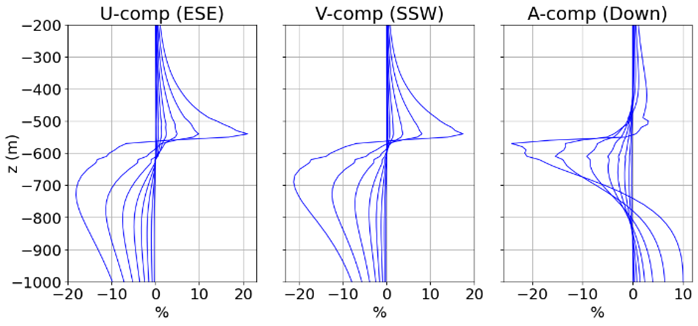
\includegraphics[width=0.65\columnwidth]{images/utem_bh1.png}
\vspace{-5pt}
\caption{Channel reduced data for BH-1.}
\label{fig:utem_bh1}
\vspace{5pt}
\end{figure}

\begin{figure}
\centering
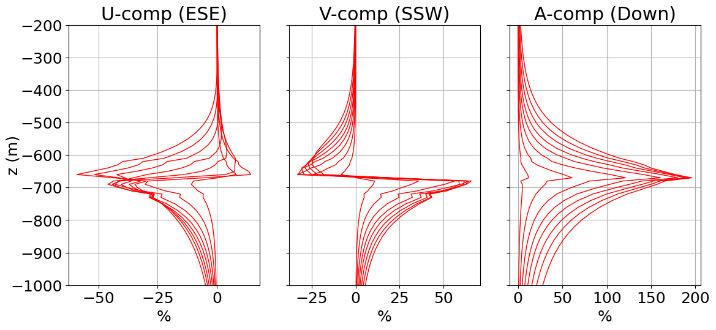
\includegraphics[width=0.65\columnwidth]{images/utem_bh2.png}
\vspace{-5pt}
\caption{Channel reduced data for BH-2.}
\label{fig:utem_bh2}
\vspace{5pt}
\end{figure}

\begin{figure}
\centering
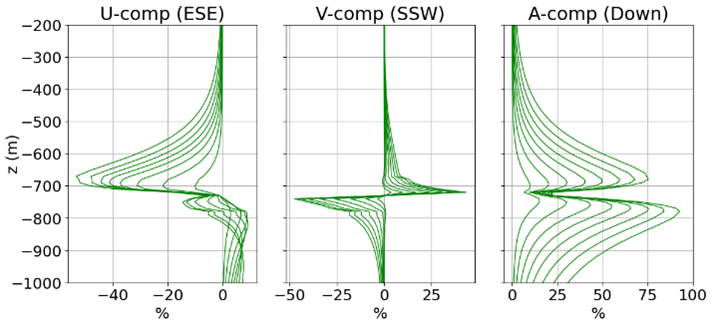
\includegraphics[width=0.65\columnwidth]{images/utem_bh3.png}
\caption{Channel reduced data for BH-3.}
\label{fig:utem_bh3}
\end{figure}

%========================================================
\section{Conclusion}
%========================================================

We developed a hierarchical FV approach for simulating inductive TDEM data in the presence of thin, highly conductive structures. By parameterizing the electrical properties to mesh cells, faces (and edges), both host and target structures can be conductively inhomogeneous and geometrically complex. The hierarchical FV formulation has demonstrated the ability to better preserves the physics of the forward simulation compared to plate-modeling software, while using a fraction of the computational resources required for standard 3D voxel approaches. Additionally, the numerical scheme remains stable as conductances exceed 1e4 S. The hierarchical FV formulation offers a generalized approach that accounts for inhomogeneity and irregular geometry in both host and target structures. The impact of the hierarchical FV formulation is the ability to perform hypothesis testing for geologically realistic hypotheses when thin conductive targets are present. Future work aims to use the hierarchical FV formulation to construct and solve parameter estimation problems.



% For bibliography
\onecolumn
\bibliographystyle{seg} % style file is seg.bst
\bibliography{bibliography}
\end{document}




